\chapter{Turbine a flusso assiale e misto}
Nel caso delle turbine non si parlerà di flusso assiale puro, è presente anche una significativa componente radiale. Nel caso di una turbina il salto entalpico per stadio è di gran lunga superiore all'analogo elaborabile dal compressore. Entalpia e temperatura decrescono molto rapidamente, l'ipotesi di avere densità costante e l'andamento delle pressioni a gradino tra stadi successivi non è più accettabile a causa proprio della dimensione del salto entalpico. Abbiamo temperature molto elevate, nel compressore è la qualità del design del profilo a dominare mentre nella turbina il limite costruttivo è dato dai materiali della palettatura che lavorano a temperature molto elevate e con deflessioni che vanno dai $50^{\circ} a 180^{\circ}$. 
\begin{figure}[h!]
\centering
  \includegraphics[width=.9\textwidth]{fig/TurboGas.png}
\caption{}
\label{fig:TurboGas}
\end{figure}
Il proilo aerodinamico utilizzato in un compressore sarà quindi molto diverso da quello utilizzato in una turbina, quest'ultimo rappresenta più una effettiva variazione di condotto. 
Per andare a vedere come si presenta una turbina assiale facciamo riferimento all'immagine in figura \ref{fig:TurboGas}, è rappresentata una turbina a gas ad uso terrestre. Le pale sono attorno ai 45 gradi, immaginando la parte statorica si avrà un grado di reazione di 0.5, probabilmente ad eccezione del primo stadio, a monte potrebbe esserci un IGV. Sono presenti $17$ stadi di compressione e solo $3$ di turbina. 

Vediamo allora quali possono essere le varie configurazioni di turbina. 
Vi sono innanzitutto gli stadi ad azione $R = 0$
\begin{align*}
\begin{cases}
\mbox{De laval}, & z_v = 1\\
\mbox{Curtis}, & z_v = 2 \div 3\\
\mbox{Reteau}, & z_v = 1\\
\end{cases}
\end{align*}
Con $z_v$ salti di velocità. Ci sono poi le turbine Parsons con $R = 5$. Si possono così andare a determinare i triangoli di velocità.

\begin{align*}
\bigg( \frac{u}{c_1} \bigg)_{opt} = \frac{\sin \alpha_1}{2 z_v}, \; \mbox{per} \; R = 0
\end{align*}
\begin{align*}
\bigg( \frac{u}{c_1} \bigg)_{opt} = \sin \alpha_1, \; \mbox{per} \; R = 0.5
\end{align*}
Poi essento $\alpha_1$ piccolo si può scrivere $ \sin \alpha_1 \simeq \alpha_1$ semplificando ulteriormente le espressioni.

\section{Calcolo dei rendimenti}
Andiamo ora a vedere quello che succede all'interno dello stadio di una turbina. Mi pongo su un sistema di riferimento con linea media del condotto palare come mostrato in \ref{fig:SezioneTurbina}. Non posso più assumere trascurabile la variazione di raggio. 
\begin{figure}
\centering
\begin{minipage}{.5\textwidth}
  \centering
  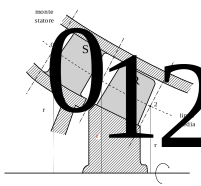
\includegraphics[width=.95\linewidth]{fig/SezioneTurbina.pdf}
  \captionof{figure}{}
  \label{fig:SezioneTurbina}
\end{minipage}%
\begin{minipage}{.5\textwidth}
  \centering
  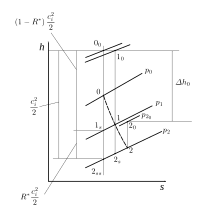
\includegraphics[width=.95\linewidth]{fig/hsturbine.pdf}
  \captionof{figure}{}
  \label{fig:hsturbine}
\end{minipage}
\end{figure}
Il salto entalpico tra i punti $1 - 2_s$ è leggermente superiore a quello presente tra i punti $1_s - 2_{ss}$ questo a causa della divergenza delle isobare. A tal proposito si introduce il fattore di recupero $f$ 
\begin{align*}
(1- R^*) \cdot \frac{c_i^2}{2}
\end{align*}
\begin{align*}
(1+f)r^* \cdot \frac{c_i^2}{2} \; \mbox{salto tra $1$ e $2_s$}
\end{align*}
Questo fattore di recupero è fisicamente spiegabile dal fatto che la trasformazione non essendo puramente isoentropica causa un aumento della temperatura parzialmente recuperabile nell'attraversamento successivo. 

\subsection{Rendimenti}
Il rendimento è il seguente
\begin{align*}
\eta = \cfrac{h_{0_0} - h_{0_2}}{h_{0_0} - h_{2_{ss}} - \Phi_E \cfrac{c_2^2}{2}} = \frac{\Delta h_0}{\Delta h_{is_{ts}}-\Phi_E \cfrac{c_2^2}{2}}
\end{align*}
Il termine fi e rappresenta la quota cinetica a valle della turbina. Quando lo considero uguale a 1 sto considerando un rendimento total to total mentre se lo considero pari a zero sto considerando un rendimento total to static.
\begin{align*}
\begin{cases}
\Phi_E = 1 \; \Rightarrow & \eta = \eta_{tt}\\
\Phi_E = 0 \; \Rightarrow & \eta = \eta_{ts}
\end{cases} 
\end{align*}
Seguono ora una serie di definizioni. Cifra di lavoro
\begin{align*}
\psi = \cfrac{h_{0_0} - h_{2_{ss}}}{\cfrac{u^2}{2}} = \frac{c_1^2}{u_1^2} = \frac{\Delta h_{is_{ts}}}{\cfrac{u^2}{2}}
\end{align*}
Coeiciente di portata
\begin{align*}
\Phi_1 = \frac{c_{m1}}{u_1}
\end{align*}
Grado di reazione
\begin{align*}
R^* = \frac{h_{1s} - h_{2ss}}{h_{0_0} - h_{2_{ss}}} = \frac{\Delta h_{Ris}}{\Delta h_{ists}}
\end{align*}
Energia cinetica totale
\begin{align*}
\frac{c_i^2}{h_{0_0} - h_{2_{ss}}}
\end{align*}
Coeiciente di velocità periferica
\begin{align*}
k_{is} = \frac{u_1}{c_1} = \frac{1}{\sqrt{\psi}}
\end{align*}
Coefficiente di lavoro specifico totale
\begin{align*}
\lambda = \cfrac{h_{0_0} - h_{2_0}}{\cfrac{u^2}{2}} \frac{\Delta h_0}{\frac{u^2}{2}}
\end{align*}
Voglio cercare la relazione tra il grado di reazione ideale e quello effettivo. Adimensionalizzo i triangoli di velocità. Ora non posso più riferirmi ad una sola velocità meridiana, questa diventa una grandezza di progettazione in quanto definisce le sezioni della macchina. Utilizzo quindi i rapporti tra velocità meridiane e tra i raggi.
\begin{align*}
\frac{c_{m2}}{c_{m1}}, \;\; \frac{r_2}{r_1}
\end{align*}
Adimensionalizzo tutte le grandezze con la velocità periferica $u_1$. Chiaramente i triangoli di velocità saranno di dimensioni diverse. 
\begin{figure}[h!]
\centering
  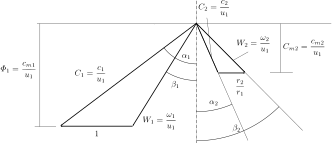
\includegraphics[width=.8\textwidth]{fig/triangTurb.pdf}
\caption{}
\label{fig:triangTurb}
\end{figure}
Posso ora andare a sviluppare l'espressione del rendimento
\begin{equation}
\eta = \cfrac{\Delta h_0}{\Delta h_{is_{ts}} - \Phi_E \cfrac{c_2^2}{2}} \cdot \frac{\frac{1}{u_1^2/2}}{\frac{1}{u_1^2/2}} = \frac{\lambda}{\psi - \Phi_E \left( C_2^2 \right)}
\end{equation}
Espandendo il numeratore
\begin{align*}
\lambda = \cfrac{\Delta h_0}{\cfrac{u_1^2}{2}} = \frac{2 \left( u_1 c_{u1} - u_2 c_{u2} \right)}{u_1^2} = 2 \bigg( C_{u1} - \frac{r_2}{r_1} C_{u2} \bigg)
\end{align*}
Scrivo ora le velocità assolute adimensionalizzate in funzione del rendimento e del grado di reazione. 
\begin{align*}
\frac{c_1^2}{2} = \left( 1 - R^* \right) \frac{c_i^2}{2} \cdot \eta_s \; \Rightarrow \; c_1 = \sqrt{\eta_s \left( 1 - R^* \right)} \cdot c_i
\end{align*}
\begin{align*}
C_1 = \frac{c_1}{u_1} = \sqrt{\eta_s \left(1- R^* \right)} \cdot \frac{c_i}{u_1}, \; \mbox{con } \frac{c_i}{u_1} = \frac{1}{k_{is}}
\end{align*}
Ottengo
\begin{equation}
\boxed{ C_1 = \frac{\sqrt{\eta_s}}{k_{is}} \sqrt{1 - R^*} }
\end{equation}
Vado a vedere la stessa cosa per le altre grandezze. Per espandere la velocità relativa adimensionalizzata utilizzo il teorema di Carnot
\begin{align*}
W_1^2 = C_1^2 + 1^2 - 2 \cdot 1 \cdot C_1 \cos \big( \frac{\pi}{2} - \alpha_1 \big)
\end{align*}
ottengo
\begin{align*}
\boxed{ W_1 = \sqrt{1 + \frac{n_{is}}{k_{is}^2} \left( 1 - R^* \right) - 2 \frac{\sqrt{\eta_s}}{k_{is}} \sqrt{1-R^*} \cdot \sin \alpha_1}}
\end{align*}
Per quanto riguarda $W_2$. Considero il salto entalpico e lo scrivo in funzione del fattore di recupero
\begin{equation}
h_2 - h_1 = \frac{u_2^2 - u_1^2}{2} - \frac{\omega_2^2 - \omega_1^2}{2}
\end{equation}
\begin{align*}
h_1 - h_2 = \frac{c_i^2}{2} \cdot R^* \left( 1 + f \right) \eta_R
\end{align*}
\begin{align*}
\left. \frac{\omega_2^2 - \omega_1^2}{2} - \frac{u_2^2 - u_1^2}{2} = \frac{c_i^2}{2} \cdot R^* \left( 1 + f \right) \eta_R \; \; \cdot \middle/ \frac{1}{u_1^2} \right.
\end{align*}
\begin{equation}
\boxed{W_2 = \sqrt{\frac{\eta_R \left( 1 + f \right) R^*}{k_{is}^2} + \frac{\eta_s}{k_{is}^2}  \left(1 + R^* \right) - \frac{2 \sqrt{\eta_s}}{k_{is}} \sqrt{1 - R^*} \sin \alpha_1 + \bigg(\frac{r_2}{r_1} \bigg)^2 } }
\end{equation}

Per quanto riguarda $C_{m2}$ 
\begin{align*}
c_{m2} = c_{m1} \frac{c_{m2}}{c_{m1}} c_1 \cos \alpha_1 \cdot \frac{c_{m2}}{c_{m1}}
\end{align*}
\begin{align*}
C_{m2} = C_1 \cos \alpha_1 \cdot \frac{c_{m2}}{c_{m1}}
\end{align*}
ottengo
\begin{equation}
\boxed{C_{m2} = \frac{c_{m2}}{c_{m1}} \frac{\sqrt{\eta_s}}{k_{is}} \sqrt{1 - R^*} \cos \alpha_1 }
\end{equation}
Sono in grado essenzialmente di scrivere il rendimento come funzionale di tutte le grandezze viste 
\begin{align*}
\eta = f \bigg( \psi, \Phi_R, R^*, k_{is}, f, \frac{c_{m2}}{c_{m1}}, \frac{r_2}{r_1}, \alpha_1, \eta_s, \eta_R \bigg)
\end{align*}
I primi quattro parametri sono parametri unzionali, $f$ dipende dalla divergenza delle isobare e quindi dalla natura del fluido, i tre parametri successivi sono parametri di progetto e infine gli ultimi due sono parametri della schiera rotorica e statorica.
Possiamo tracciare un diagramma di rendimento total - static / total - total in funzione della cifra di lavoro. 
\begin{figure}
\centering
  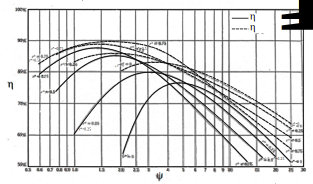
\includegraphics[width=.8\textwidth]{fig/Rendimenti_ts_tt.pdf}
\caption{}
\label{fig:Rendimenti_ts_tt}
\end{figure}
\section{Proprietà termodinamiche del flusso}
Si possono ora andare a calcolare le proprietà termodinamiche del flusso nell'attraversamento della turbina. Si definisce il numero di Mach periferico come segue
\begin{align*}
M_u = \frac{u_1}{a_{0_0}}
\end{align*}
Posso però esprimere la velocità acustica a monte della turbina in funzione dell'entalpia totale
\begin{align*}
a_{0_0} = \sqrt{kRT_{0_0}} = \sqrt{\frac{c_p}{c_v} \left( c_p - c_v \right) T_{0_0}} = \sqrt{h_{0_0} \left( k - 1 \right)}
\end{align*}

\begin{align*}
\psi	= \cfrac{h_{0_0} - h_{2ss}}{\cfrac{u_1^2}{2}} = \cfrac{c_i^2}{u_1^2} = \cfrac{\Delta h_{is_{ts}}}{\cfrac{u_1^2}{2}}
\end{align*}

\begin{align*}
\frac{c_i^2}{2} = \psi \frac{u_1^2}{2} \frac{a_{0_0}^2}{a_{0_0}^2} = \frac{\psi}{2} Mu^2 (k-1) h_{0_0}
\end{align*}
\begin{align*}
h_{1s} = h_{0_0} - \left(1- R^* \right) \frac{c_i^2}{2} = h_{0_0} \bigg[ 1- \left( 1- R^* \right) \frac{k-1}{2} \psi M_u^2 \bigg]
\end{align*}
\begin{align*}
h_{2ss} = h_{0_0} - \frac{c_i^2}{2} = h_{0_0} \bigg[ 1 - \frac{k-1}{2} \psi M_u^2 \bigg]
\end{align*}

\begin{align*}
\frac{c_1^2}{2} = \eta_s \frac{c_i^2}{2} \left( 1- R^* \right)
\end{align*}
\begin{align*}
h_1 = h_{0_0} - \frac{c_1^2}{2} = h_{0_0} \bigg[ 1- \left( 1- R^* \right) \frac{k-1}{2} \eta_s \psi M_u^2 \bigg]
\end{align*}

\begin{align*}
h_2 = h_{0_0} - \Delta h_0 - \frac{c_2^2}{2} = h_{0_0} \bigg[ 1- \bigg( \eta_{ts} + \frac{C_2^2}{\psi} \bigg) \frac{k-1}{2} \psi M_u^2 \bigg]
\end{align*}
